\documentclass{article}

\newcommand{\PRETTY}{}

\usepackage[pdftex]{graphicx}
\usepackage{tikz}
\usetikzlibrary{arrows, shapes, backgrounds, chains, decorations, calc, fit,
    shadows, external}
\tikzexternalize
\tikzset{external/force remake}
\usepackage{pgf}
\usepackage{tikzuml-v1.0b/tikz-uml}
\usepackage[english]{babel}

\tikzset{
  node distance=1.5cm,
  every node/.style={align=center}
}

\begin{document}
%\input figures/workspace.tikz
\begin{tikzpicture}[node distance=1.5cm, every node/.style={align=center}]
\input figures/git-model-base.tikz
\end{tikzpicture}

\begin{tikzpicture}[node distance=1.5cm, every node/.style={align=center}]
\input figures/git-model-base.input
\begin{pgfonlayer}{background}
  \node[ellipse, fill=black!20, fit=(tr1_1) (b1_2) (b1_3), xscale=0.75,
  yshift=-0.5cm]{};
  \node[ellipse, fill=black!20, fit=(tr2_1) (b2_2) (b2_4)]{};
\end{pgfonlayer}
\end{tikzpicture}

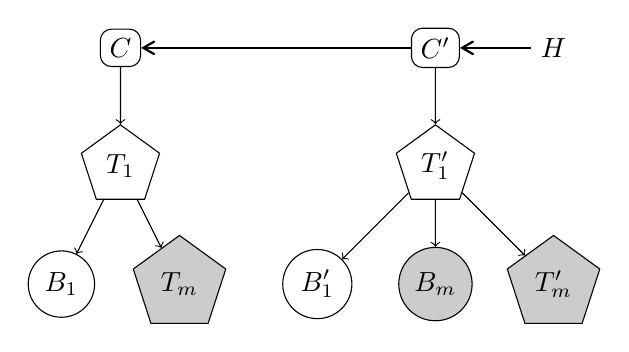
\begin{tikzpicture}
\tikzstyle{commit}=[rectangle, draw, rounded corners]
\tikzstyle{tree}=[regular polygon, regular polygon sides=5, draw, thin]
\tikzstyle{blob}=[circle, draw, thin]

% mock tree/blob object
\tikzstyle{mock_tree}=[regular polygon, regular polygon sides=5, draw, thin,
  fill=black!20]
\tikzstyle{mock_blob}=[circle, draw, thin, fill=black!20]

\tikzstyle{parent}=[-angle 60, draw, thick]
\tikzstyle{edge from parent}=[->, draw]
\tikzstyle{2obj}=[->, draw]
% tree 1
\node[commit](ci1){$C$}
child{node[tree](tr1){$T_1$}
  child{node[blob](b1_1){$B_1$}}
  child{node[mock_tree](tr1_1){$T_m$}}
};

% tree 2
\node[commit, right of=ci1, node distance=4cm](ci2){$C'$}
child{node[tree](tr2){$T'_1$}
  child{node[blob](b2_1){$B'_1$}}
  child{node[mock_blob](b2_4){$B_m$}}
  child{node[mock_tree](tr1_1){$T'_m$}}
};

\draw[parent](ci2) to (ci1);


% HEAD
\node[rectangle, right of=ci2](head){$H$};
\draw[parent](head) to (ci2);


\end{tikzpicture}


\usetikzlibrary{shapes, shadows, fit, arrows, positioning}
\tikzstyle{object} = [draw, rectangle, rounded corners, align=center, minimum
height=1cm]
\tikzstyle{new} = [fill=black!20]
\tikzstyle{pack} = [object, minimum width=35mm]
\tikzstyle{comp} = [draw, rectangle, minimum height=1cm, minimum width=0.6cm,
  very thick]
\tikzstyle{filter} = [draw, diamond, very thick]
\tikzstyle{view} = [draw, tape, tape bend top=none, double copy shadow, fill=white, minimum
height=1cm, minimum width=0.6cm, very thick]
\tikzstyle{box} = [rectangle]
\tikzstyle{network} = [draw, cloud, cloud puffs=61, fill=white, minimum width=7cm]
\tikzstyle{olist} = [->, thin, sloped]
\tikzstyle{consume} = [single arrow, midway, draw, sloped, align=center,
  minimum height=5mm, single arrow head extend=1mm]
\tikzstyle{stream} = [single arrow, draw, sloped, minimum height=3mm, single
  arrow head indent=1mm, single arrow head extend=2mm]
\tikzstyle{stream2} = [stream] %, shape border rotate=180]
\tikzstyle{vlabel} = [anchor=south, rotate=-90]

\ifdefined\PRETTY
  \tikzset{object/.append style={top color=black!20, draw=black!30, drop
      shadow, text=black!80}}
  \tikzset{new/.append style={top color=white, middle color=yellow!50!red,
     drop shadow, draw=red!50, text=red!50!black}}
  \tikzset{network/.append style={bottom color=gray, top color=white,
      drop shadow, draw=black!60, text=blue!50!black}}
  \tikzset{comp/.append style={drop shadow, fill=blue!20, draw=blue!10,
      text=blue!40!black!50}}
  \tikzset{stream/.append style={drop shadow, top color=green!30,
      draw=green!50}}
  \tikzset{consume/.append style={drop shadow, fill=yellow!50!red,
      draw=yellow}}
  \tikzset{vlabel/.append style={font=\large\scshape, text=black!60}}
\fi

\begin{tikzpicture}
  \node[matrix, label={above:Server Repository}, column sep=2mm](repo)
  {
    \node[object](obj1){loose\\object}; &
    \node[object](obj2){loose\\object}; &
    \node[pack, minimum width=45mm](obj4){pack file}; \\
  };

  \node[comp, below=1cm of repo.west, anchor=north west](revlist){\verb|git|\\\verb|rev-list --all --objects|};
  \node[filter, new, below of=revlist, node distance=1.5cm](f){filter};
  \node[view, new, anchor=west](v) at(revlist.west |- f){subdirs};
  \node[comp, below =3.5cm of revlist.east, anchor=east](gitpack){Git object packing};
  \node[box, fit= (gitpack)(repo)](server){};
  \node[vlabel, anchor=north] at (server.east){Server};

  % client side
  \node[pack, below= 3.2cm of gitpack](pack){pack file};
  \node[object, left = 2mm of pack.west, anchor=east](mockobj){mock\\objects};
  \node[object, right=2mm of pack.east, anchor=west](newobj){new\\commits};
  \node[comp, new, below =5mm of newobj](ci-ctor) {Commit\\Creator};
  \node (x) at (obj4.south-|newobj){};
  \path(newobj) to node[stream2, minimum height=8cm, pos=.48]{git push}(x);
  \node[comp, new, above=5mm of mockobj](mockc){Mock object\\builder};
  \node[comp, anchor=west, minimum width=45mm] (idx) at (mockobj.west |- ci-ctor) {Git \emph{Index}};
  \draw[olist] (idx) -- (ci-ctor);
  \draw[olist] (pack) -- (ci-ctor);
  \path(ci-ctor) to node[stream]{} (newobj);

  \node[box, fit=(mockc)(ci-ctor)](c){};
  \node[vlabel] at (c.east) {Client};
  \draw[thick](repo.south east) -- (repo.south west);

  \path(v) to node[consume, minimum width=3mm]{} (f);
  \draw[olist](obj1.south) -- (revlist);
  \draw[olist](obj2.south) -- (revlist);
  \draw[olist](obj4.south) -- (revlist);
  \draw[olist](revlist) -- (f);

  \draw[olist](f) to node{real obj\\list} (gitpack);
  \draw[olist](f) to [in=90, out=-140] node[near start]{mock obj\\list} (mockc);
  \path(gitpack) to node[stream2, minimum height=30mm, pos=.5, label={[above]45:git fetch}]{}
     node [network, aspect=3, pos=.3]{Network} (pack);
  \path(mockc) to node[stream] {} (mockobj);
%  \node[draw, single arrow, minimum height=3cm, align=left, text justified] at (0, 0){test\\1};
\end{tikzpicture}


%!tikz editor 1.0
%!tikz source begin
\begin{tikzpicture}
\begin{umlseqdiag}
\umlobject[class=Client]{c}
\umlobject[class=Server]{s}
\begin{umlcall}[op={git-upload-pack}]{c}{s}
  \begin{umlcall}[op={$H_s$}, type=return]{s}{c}
  \end{umlcall}
  \begin{umlcall}[op={$<H_w, H_h>$}, return={pack stream}]{c}{s}
    \begin{umlcall}[op={pack-objs}]{s}{s}
    \end{umlcall}
  \end{umlcall}
\end{umlcall}
\end{umlseqdiag}
\end{tikzpicture}
%!tikz source end


%!tikz editor 1.0
%!tikz source begin
\begin{tikzpicture}
\begin{umlseqdiag}                                                             
\umlobject[class=Client]{c}                                                    
\umlobject[class=Server]{s}                                                    
\begin{umlcall}[op={git-upload-pack}, return={pack stream}]{c}{s}
    \begin{umlcall}[op={$H_S$}, type=return]{s}{c}
    \end{umlcall} 
    \begin{umlfragment}[type=loop]
        \begin{umlcall}[op={dir}]{c}{s}
        \end{umlcall}
        \begin{umlcall}[op={$D_S$}, type=return]{s}{c}
        \end{umlcall}
    \end{umlfragment}
    \begin{umlcall}[op={$<H_h, H_w, D_i, D_e>$}]{c}{s}
    \end{umlcall}
    \begin{umlcall}[op={pack_objs($[H_s, H_c), D_i, D_e$)}]{s}{s}
    \end{umlcall}                 
\end{umlcall}  
\end{umlseqdiag}
\end{tikzpicture}
%!tikz source end


\end{document}
